\begin{figure}[H]
\centering


\tikzset{every picture/.style={line width=0.75pt}} %set default line width to 0.75pt        

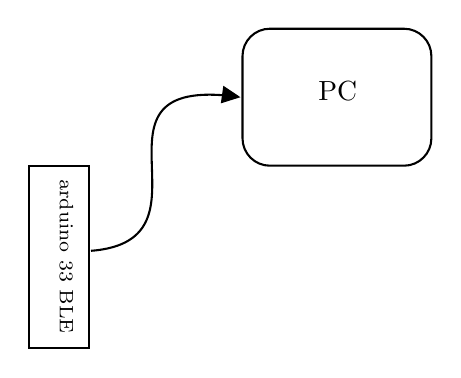
\begin{tikzpicture}[x=0.75pt,y=0.75pt,yscale=-1,xscale=1]
%uncomment if require: \path (0,528); %set diagram left start at 0, and has height of 528

%Shape: Rectangle [id:dp7327399467778912] 
\draw   (233,206) -- (233,294) -- (204,294) -- (204,206) -- cycle ;
%Rounded Rect [id:dp2315563507614331] 
\draw   (307,153.2) .. controls (307,145.91) and (312.91,140) .. (320.2,140) -- (384.8,140) .. controls (392.09,140) and (398,145.91) .. (398,153.2) -- (398,192.8) .. controls (398,200.09) and (392.09,206) .. (384.8,206) -- (320.2,206) .. controls (312.91,206) and (307,200.09) .. (307,192.8) -- cycle ;
%Curve Lines [id:da34814740280768275] 
\draw    (234,247) .. controls (298.35,242.05) and (224.51,162.61) .. (303.56,172.67) ;
\draw [shift={(306,173)}, rotate = 188.23] [fill={rgb, 255:red, 0; green, 0; blue, 0 }  ][line width=0.08]  [draw opacity=0] (8.93,-4.29) -- (0,0) -- (8.93,4.29) -- cycle    ;

% Text Node
\draw (342,164) node [anchor=north west][inner sep=0.75pt]   [align=left] {PC};
% Text Node
\draw (227,211) node [anchor=north west][inner sep=0.75pt]  [rotate=-90] [align=left] {{\scriptsize arduino 33 BLE}};
\end{tikzpicture}
\caption{ Diagrama del circuito.}
\label{fig4}
\end{figure}